\documentclass[12pt,notitlepage]{article}
\usepackage[utf8]{inputenc}
\usepackage{amsmath, amssymb}
\usepackage{geometry}
\geometry{a4paper, margin=1in}
\usepackage{listings}
\usepackage{tocloft}
\usepackage{graphicx}
\usepackage{caption}
\usepackage{enumitem}
\usepackage{xcolor} % Added for color support in listings
\usepackage{hyperref} %

\begin{document}


Gary Hobson\\
MAT 300 Module 6 Homework

\subsection*{a) Fit this model to the 12 data points given in the table, and find the regression residuals}

Using Minitab, the fitted linear model is 
\[ \text{DEMAND} = 99.8 + 0.0452 \times \text{PRICE}. \]
The residuals are:

\begin{table}[h]
    \centering
    \small % Reduce font size to make the table more compact
    \setlength{\tabcolsep}{4pt} % Reduce space between columns
    \caption{Predicted Values and Residuals for Demand Regression}
    \label{tab:demand_residuals}
    \begin{tabular}{|c|c|c|c|}
        \hline
        \textbf{PRICE} & \textbf{DEMAND} & \textbf{Predicted (\(\hat{y}\))} & \textbf{Residual} \\
        \hline
        100 & 130 & 104.33 & 25.67 \\
        700 & 150 & 131.43 & 18.57 \\
        450 & 60 & 120.14 & -60.14 \\
        150 & 120 & 106.59 & 13.41 \\
        500 & 50 & 122.40 & -72.40 \\
        800 & 200 & 135.95 & 64.05 \\
        70 & 150 & 102.98 & 47.02 \\
        50 & 160 & 102.08 & 57.92 \\
        300 & 50 & 113.37 & -63.37 \\
        350 & 40 & 115.62 & -75.62 \\
        750 & 180 & 133.69 & 46.31 \\
        700 & 130 & 131.43 & -1.43 \\
        \hline
    \end{tabular}
\end{table}

\subsection*{b) Plot the residuals against retail price per carat, \( x \)}

The residual vs.\ PRICE plot shows residuals starting positive at low prices (50--150), becoming negative at moderate prices (300--500), and returning to positive at high prices (700--800), forming a U-shape.

\subsection*{c) Can you detect any trends in the residual plot? What does this imply?}

The residual plot exhibits a U-shaped trend, indicating the linear model is inadequate. This suggests a quadratic model (\( y = \beta_0 + \beta_1 x + \beta_2 x^2 \)) is needed to capture the theorized demand behavior (decreasing at low prices, leveling off at moderate prices, increasing at high prices).



\begin{figure}[h]
    \centering
    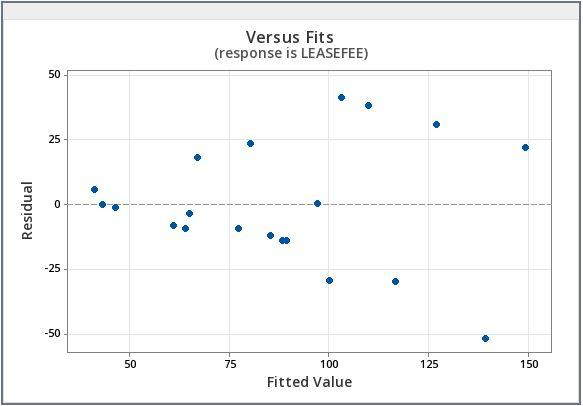
\includegraphics[width=0.8\textwidth]{Residual_vs_Fitted.jpeg}
    \caption{residual vs. fitted}
\end{figure}







\end{document}